%!TEX root = ../../../report.tex

\subsection{Dataflow}
\newpage
When designing an energy efficient system, dataflow is of great importance. The
software on the MCU has been designed to minimize the number of data stores and
movements. When possible, DMA was utilized to move the data while running in a
low power mode. The dataflow consist of four phases, as shown in figure \ref{sw_transfer_phases}. 
In phase 1 the MCU acquires input samples from an input device. These samples are 
then transfered to the FPGA in phase 2. When the FPGA is finished processing the
samples, they are transfered back to the MCU in phase 3. In the last phase the MCU
sends the filtered samples to an output device. All these phases are executed 
concurrenlty to ensure a constant flow of samples. The phase 2 and 4 are constant, 
while the first and the last flow changes depending on the I/O devices selected. 

\begin{figure}[H]
	\centerline{
	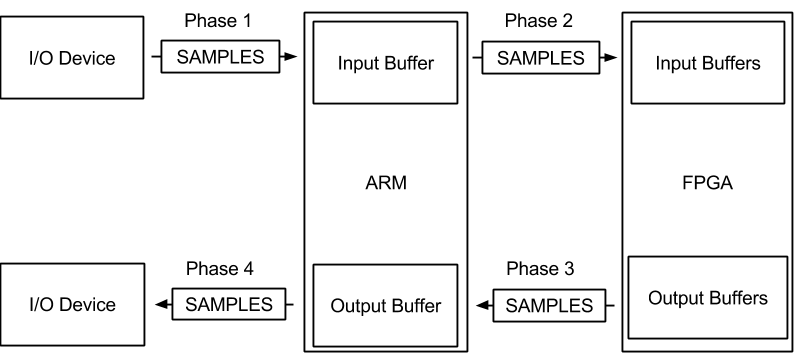
\includegraphics[width=400px]{figures/sw/transfer-phases.png}}
	\caption{Transfer Phases}
	\label{fig:sw_transfer_phases}
\end{figure}
\FloatBarrier


\subsubsection{Direct Memory Access} DMA provides the ability to move data
without the intervention of the CPU. This is used extensively to implement the
dataflow when the MCU is running in a low energy mode. The CPU is only used to configure
and refresh the DMA channels in between transfers. The MCU provides 12
independent DMA channels which can move data between peripherals, Internal RAM, and
devices connected to EBI, like the FPGA.

The main flow of data goes from Internal RAM on the MCU to the buffers on
the FPGA, and back to Internal RAM on the MCU. This dataflow path is illustrated in figure.

% \input{figures/sw/ram-fpga-ram}

\paragraph{Deinterleaving of Samples}
When reading from both a WAV file or the ADC, samples from the stereo channels
are interleaved. The FPGA handles each channel in separate pipelines. As shown 
in figure \ref{fig_sw_main_dataflow}. 
When reading the samples they have to be deinterleave. Deinterleaving is the
process of splitting the samples for each channels in to two separate streams. 
The complementary operation of interleaving the samples is performed before the samples 
are moved to the output peripherals.
\missingfigure{Figure showing deinterleaving and interleaving}

This is implemented with two version. One using only the CPU and one using DMA transfers
while the CPU is sleeping. Comparions of the two methods are included in the results section.
\todo{Make sure they are. Rewrite for better flow - JK}

The samples are de-interleaved by letting two DMA channels read from the same
source and write to the correct pipeline for the correct channel. The first DMA
copies the samples for the left stero channel, and start without a offset. The
second DMA copies the samples for the right stereo channel and start with an
offset of one sample. Both DMAs read only every second sample and writes them
continuously to the FPGA input buffers.

The interleaving process on output side works in the same way. The DMA reading
from the pipeline containing the left stereo channel samples writes to the
memory without a starting offset. The right channel DMA writes with an offset by
one sample.
\todo[inline]{Rewrite for better flow - JK}

\paragraph{}
In addition, a DMA is assigned for each ADC and DAC whenever they are used as
input and output, respectively. When SDCard is used, the contents of the files
are read and written directly to and from RAM by the CPU.


\subsubsection{Peripherals}

\begin{figure}[h]
	\centering
	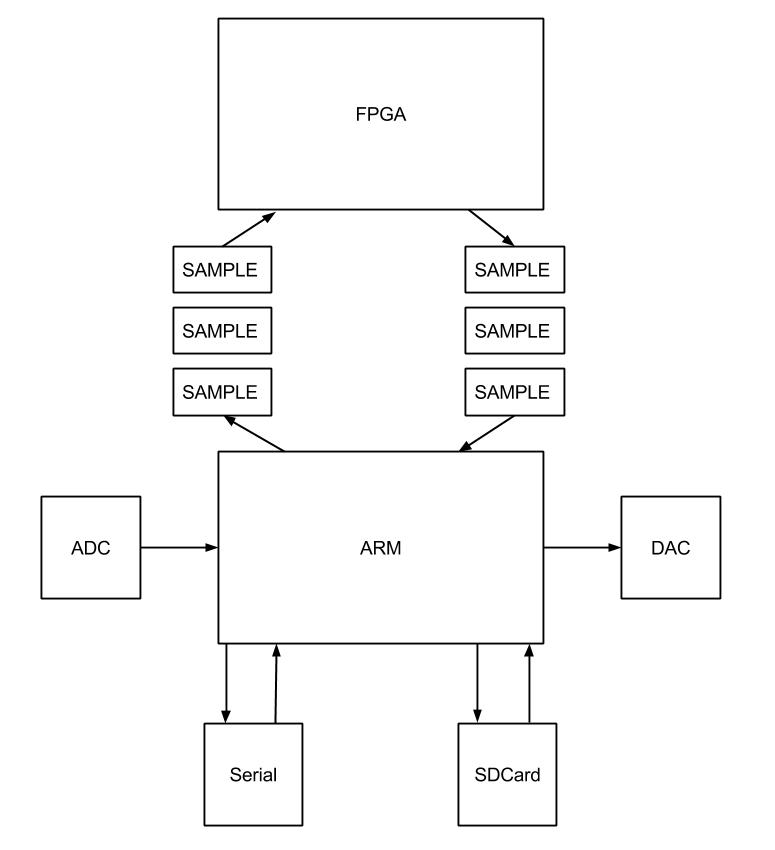
\includegraphics[height=150px]{figures/sw/sample-flow.png}
	%\begin{tikzpicture}[shorten >= 1pt, node distance=3cm, on grid, auto]
	%	\node[draw,rectangle,minimum size=2cm] (fpga) {FPGA};
	%	\node[draw,rectangle,below of=fpga,minimum size=2cm] (arm) {ARM};
	%\end{tikzpicture}
	\caption{Flow of samples}
	\label{fig:sw_sample_flow}
\end{figure}
\todo{Tikzify}

Figure \ref{fig:sw_sample_flow} shows all the peripherals included in flow of sample. 
These are ADC, DAC, SDCard and the FPGA. The ADC and DAC are connected to the Minijack
audio ports on the circuit board and directly linked to GPIO ports on the MCU. The SDCard
is mounted on the board and connected to the MCU through the SPI, Serial Peripheral Interface
bus. Lastly the FPGA is connected to the MCU on the EBI.

\subsubsection{External Bus Interface}
The MCU is connected to the FPGA and External SRAM through the EBI. This is a standard
bus interface provided by the MCU. Utilizing the EBI leads to a
simple interface with these units as the bus is memory mapped on the MCU.
Communicating with the FPGA is done by reading and writing to memory.
The EBI bus is initialized by the {\it emlib} software library.

\subsubsection{Serial Peripheral Interface}
The SPI bus is a general bus interface used by many embedded applications. It is used
for the communication bewteen the MCU and a MicroSD memory card connected to the slot
on the board \ref{} \todo{Har vi bilde av bitless?}. 

\subsubsection{General Purpose Input/Output}
To capture a audio stream from the input Minijack, one GPIO pin is connected to a 
ADC, Analog to Digital Converter, on the MCU. The ADC measures the the 

\todo{more about how the bus is implemented on the MCU}

\paragraph{Triggering Transfers}

All the DMA transfers are triggered by the use of one clock, the sample clock.
This clock is run at the sample speed 11 kilohertz when using the DAC or ADC. Or
an arbitrary frequency when sampling from SD to SD. The clock signal is fed into
the Peripheral Reflex System (PRS) of the MCU and propagates through the system
using the following scheme

%\newpage %re-insert if figure breaks across pages
\begin{verbatim}
                        | Audio in
                        V
+------+  +-----+    +------+   +-----+     +--------+
|TIMER0|->| PRS |-+->| ADC0 |-->| DMA |---->| Buffer |
+------+  +-----+ |  +------+   +-----+     +--------+
                  |     .                      / \
                  |     .                     /   \
                  |     .                    V     V
                  |     .              +-----+     +-----+
                  |     +....irq......>| DMA |....>| DMA |
                  |                    +-----+     +-----+
                  |                       |           |
                  |                       V           V
                  |                   +------+    +-------+
                  |                   | FPGA |    | FPGA  |
                  |                   | Left |    | Right |
                  |                   +------+    +-------+
                  |                       |           |
                  |                       V           V
                  |                    +-----+     +-----+
                  |     +....irq......>| DMA |....>| DMA |
                  |     .              +-----+     +-----+
                  |     .                    \     /
                  |     .                     \   /
                  |     .                       V
                  |  +------+   +-----+     +--------+
                  +->| DAC0 |<--| DMA |<----| Buffer |
                     +------+   +-----+     +--------+
                        |
                        V Audio out
\end{verbatim}

Here, both the DAC and ADC consumes the PRS signal originated from TIMER0. The
DMA copying from the ADC to the RAM buffer, and the two DMAs performing the
de-interleaving of the input samples, receive a pulse each time the ADC has
buffered $N$ samples. They then perform a sequence of copy actions resulting
in the input samples ending up inside the pipeline buffers of the FPGA. On the
other side the DAC sends a pulse to the DMA that feeds it samples in conjunction
with the two DMAs performing the interleaving of the samples returned from the
FPGA pipelines.
